\documentclass[a4paper, 12pt]{article}		% general format
\usepackage{multicol}
%%%% Charset
\usepackage{cmap}							% make PDF files searchable and copyable
\usepackage[utf8x]{inputenc} 				% accept different input encodings
\usepackage[english,russian]{babel}   %% загружает пакет многоязыковой вёрстки
\usepackage{fontspec}      %% подготавливает загрузку шрифтов Open Type, True Type и др.
\defaultfontfeatures{Ligatures={TeX},Renderer=Basic}  %% свойства шрифтов по умолчанию
\setmainfont[Ligatures={TeX,Historic}]{Roboto-Light} %% задаёт основной шрифт документа
\setsansfont{Roboto-Light}  
\usepackage{float}
%%%% Graphics
\usepackage[dvipsnames]{xcolor}			% driver-independent color extensions
\usepackage{graphicx}						% enhanced support for graphics
\usepackage{wrapfig}						% produces figures which text can flow around
\usepackage{hyperref}
%%%% Math
\usepackage{amsmath}						% American Mathematical Society (AMS) math facilities
\usepackage{amsfonts}						% fonts from the AMS
\usepackage{amssymb}						% additional math symbols

%%%% Typograpy (don't forget about cm-super)
\usepackage{microtype}						% subliminal refinements towards typographical perfection
\linespread{1.3}							% line spacing
\usepackage[left=2.5cm, right=1.5cm, top=2.5cm, bottom=2.5cm]{geometry}
\setlength{\parindent}{0pt}					% we don't want any paragraph indentation
\usepackage{parskip}						% some distance between paragraphs

%%%% Tables
\usepackage{tabularx}						% tables with variable width columns
\usepackage{multirow}						% for tabularx
\usepackage{hhline}							% for tabularx
\usepackage{tabu}
\usepackage{longtable}

%%%% Graph
\usepackage{tikz}							% package for creating graphics programmatically
\usetikzlibrary{arrows}						% edges for tikz

%%%% Other
\usepackage{url}							% verbatim with URL-sensitive line breaks
\usepackage{fancyvrb}						% sophisticated verbatim text (with box)

\usepackage{listings}
\usepackage{caption}
\DeclareCaptionFont{white}{\color{white}}
\DeclareCaptionFormat{listing}{\colorbox{gray}{\parbox{\dimexpr\textwidth-1.72\fboxsep\relax}{#1#2#3}}}
\captionsetup[lstlisting]{format=listing,labelfont=white,textfont=white,margin=0pt}
\lstset{language=C,
	basicstyle=\footnotesize,
	keepspaces=true,
	tabsize=4,               
	frame=single,                           % Single frame around code
	rulecolor=\color{black},
	captionpos=b,
	showstringspaces=false,	
	abovecaptionskip=-0.9pt,
	xleftmargin=3.4pt,
	xrightmargin=2.6pt,
	breaklines=true,
	postbreak=\raisebox{0ex}[0ex][0ex]{\ensuremath{\color{black}\hookrightarrow\space}},
	xleftmargin=3.2pt,
	literate={а}{{\selectfont\char224}}1
	{~}{{\textasciitilde}}1
	{б}{{\selectfont\char225}}1
	{в}{{\selectfont\char226}}1
	{г}{{\selectfont\char227}}1
	{д}{{\selectfont\char228}}1
	{е}{{\selectfont\char229}}1
	{ё}{{\"e}}1
	{ж}{{\selectfont\char230}}1
	{з}{{\selectfont\char231}}1
	{и}{{\selectfont\char232}}1
	{й}{{\selectfont\char233}}1
	{к}{{\selectfont\char234}}1
	{л}{{\selectfont\char235}}1
	{м}{{\selectfont\char236}}1
	{н}{{\selectfont\char237}}1
	{о}{{\selectfont\char238}}1
	{п}{{\selectfont\char239}}1
	{р}{{\selectfont\char240}}1
	{с}{{\selectfont\char241}}1
	{т}{{\selectfont\char242}}1
	{у}{{\selectfont\char243}}1
	{ф}{{\selectfont\char244}}1
	{х}{{\selectfont\char245}}1
	{ц}{{\selectfont\char246}}1
	{ч}{{\selectfont\char247}}1
	{ш}{{\selectfont\char248}}1
	{щ}{{\selectfont\char249}}1
	{ъ}{{\selectfont\char250}}1
	{ы}{{\selectfont\char251}}1
	{ь}{{\selectfont\char252}}1
	{э}{{\selectfont\char253}}1
	{ю}{{\selectfont\char254}}1
	{я}{{\selectfont\char255}}1
	{А}{{\selectfont\char192}}1
	{Б}{{\selectfont\char193}}1
	{В}{{\selectfont\char194}}1
	{Г}{{\selectfont\char195}}1
	{Д}{{\selectfont\char196}}1
	{Е}{{\selectfont\char197}}1
	{Ё}{{\"E}}1
	{Ж}{{\selectfont\char198}}1
	{З}{{\selectfont\char199}}1
	{И}{{\selectfont\char200}}1
	{Й}{{\selectfont\char201}}1
	{К}{{\selectfont\char202}}1
	{Л}{{\selectfont\char203}}1
	{М}{{\selectfont\char204}}1
	{Н}{{\selectfont\char205}}1
	{О}{{\selectfont\char206}}1
	{П}{{\selectfont\char207}}1
	{Р}{{\selectfont\char208}}1
	{С}{{\selectfont\char209}}1
	{Т}{{\selectfont\char210}}1
	{У}{{\selectfont\char211}}1
	{Ф}{{\selectfont\char212}}1
	{Х}{{\selectfont\char213}}1
	{Ц}{{\selectfont\char214}}1
	{Ч}{{\selectfont\char215}}1
	{Ш}{{\selectfont\char216}}1
	{Щ}{{\selectfont\char217}}1
	{Ъ}{{\selectfont\char218}}1
	{Ы}{{\selectfont\char219}}1
	{Ь}{{\selectfont\char220}}1
	{Э}{{\selectfont\char221}}1
	{Ю}{{\selectfont\char222}}1
	{Я}{{\selectfont\char223}}1,
	extendedchars=true
}

%галочка
\usepackage{amssymb}% http://ctan.org/pkg/amssymb
\usepackage{pifont}% http://ctan.org/pkg/pifont
\newcommand{\cmark}{\ding{52}}%
\newcommand{\xmark}{\ding{56}}
%------------------------------------------------------------------------------
\renewcommand{\labelenumii}{\theenumii}
\renewcommand{\theenumii}{\theenumi.\arabic{enumii}.}
\begin{document}
%------------------------------------------------
	\begin{titlepage}
		\begin{center}
			\large {Санкт-Петербургский политехнический университет Петра Великого\\
				Институт компьютерных наук и технологий}\\
		\end{center}
		\begin{center}
			\large\textbf {Кафедра компьютерных систем и программных технологий}
		\end{center}
		\vfill
		\begin{center}
			\large{\textbf{Отчет о лабораторной работе №5} \\
			\textbf{Курс: } Администрирование компьютерных сетей\\
			\textbf{Тема: } Перенос сети в Cisco Packet Tracer}
		\end{center}
		
		\vfill
		
		\flushleft{Выполнил студент группы 13541/3} 
		\hfill\parbox{9 cm}{\hspace*{3cm}\hbox to 0cm{\raisebox{-1em}{\small(подпись)}}\hspace*{-0.8cm}\rule{3cm}{0.8pt} Д.В. Круминьш}\\[0.6cm]
		
		\flushleft{Преподаватель} \hfill\parbox{9 cm}{\hspace*{3cm}\hbox to 0cm{\raisebox{-1em}{\small(подпись)}}\hspace*{-0.8cm}\rule{3cm}{0.8pt} И.А. Малышев}\\[0.6cm]
		
		\vspace{\fill}
		\begin{center}
			Санкт-Петербург \\ 2018 г.
		\end{center}
	\end{titlepage}
%------------------------------------------------
\setcounter{page}{2}
\tableofcontents
\clearpage

%------------------------------------------------------------------------------
%\input{intro}
\section{Постановка задачи}
В данной работе, для заданных системных функций необходимо:
\begin{enumerate}
\item ознакомиться с функциональностью и параметрами;
\item изучить исходный код;
\item произвести перехват;
\item модифицировать исходный код.
\end{enumerate}
Заданные системные функции: \textbf{fork, execve, exit}.\\
Работа будет производиться для следующих версий ядер и виртуальных систем:
\begin{itemize}
\item \textbf{4.13.0-38-generic} - \textbf{Ubuntu 16.04};
\begin{itemize}
\item glibc 2.23
\end{itemize}
\item \textbf{2.6.32-21-generic} - \textbf{Ubuntu 10.04}
\begin{itemize}
\item glibc 2.11.1
\end{itemize}
\end{itemize}
Для выполнения работы использовалась \textbf{VMware Workstation 12 pro (12.5.7 build-5813279)}

\section{Сведения о системе}
Работа производилась на реальной системе, со следующими характеристиками:
\tabulinesep = 1mm
\begin{longtabu} to \textwidth {|X[10, c , m ] |X[25, c , m ] | }\firsthline\hline

\textbf{Элемент}&\textbf{Значение}\\ \hline \endfirsthead
	
Имя ОС&Майкрософт Windows 10 Pro (Registered Trademark)\\ \hline
Версия&10.0.16299 Сборка 16299\\ \hline
Установленная оперативная память (RAM) &16,00 ГБ\\ \hline
Процессор&Intel(R) Core(TM) i5-7300HQ CPU @ 2.50GHz, 2496 МГц, ядер: 4, логических процессоров: 4\\ \hline
\caption{Сведения о системе}
\end{longtabu}

\section{Перехват системных функций}
Для осуществления перехвата будет использоваться \textbf{LKM} и создание временных отображений памяти(\textbf{MMU}).
\subsection{Linux loadable kernel module}
\textbf{LKM}(Linux loadable kernel module) - динамическое подключения/отключения модулей ядра без перекомпиляции всего ядра.

Для начала необходимо загрузить заголовки текущего ядра, для этого необходимо узнать версию используемого ядра и скачать заголовки.
\lstinputlisting[caption=Установка заголовков, language={}]{sourceCode/hook/setup.log}

Далее необходимо создать файл \textbf{Makefile}.
\lstinputlisting[caption=Makefile, language={}]{sourceCode/hook/helloWorld/Makefile}
В первой строчке указана цель сборки, в данном случае модуль \textbf{hello}. Далее указаны пути для сборки.

Далее необходимо приступить к написанию самого модуля, в данном случае он просто будет выводить текст.
\lstinputlisting[caption=hello.c, language=C]{sourceCode/hook/helloWorld/hello.c}
Важными частями модуля, являются функции определенным макросами \textbf{\_\_init} и \textbf{\_\_exit} - точки входа и выхода\cite{lkm}.

Приступаем к сборке модуля.
\lstinputlisting[caption=Лог сборки, language={}]{sourceCode/hook/helloWorld/make.log}
По завершению сборки, будет создан файл \textbf{hello.ko} - модуль для внедрения в ядро. Для подключения модуля используется команда \textbf{insmod}, а для просмотра текущих модулей, команда \textbf{lsmod}.
\lstinputlisting[firstnumber=1,firstline=1,lastline=10, caption=Внедрение и список модулей]{sourceCode/hook/helloWorld/insmod.log}
Как видно, модуль успешно встроен и функционирует.

Для выгрузки модуля используется команда \textbf{rmmod}.
\lstinputlisting[caption=Выгрузка модуля, language={}]{sourceCode/hook/helloWorld/rmmod.log}
Дополнительно посмотрим сообщения модуля, записанные в лог.
\lstinputlisting[caption=Лог сообщений модуля, language={}]{sourceCode/hook/helloWorld/kern.log}
Как видно, в лог были добавлены новые записи. В дальнейшем, на основе данного метода будут написаны перехватчики системных функций.
\subsection{Отображение в память}
Приведенное решение перехвата, основано на соответствующей статье\cite{habrHook}.

\subsubsection{Методика осуществления перехвата}
Суть описываемого способа осуществления перехвата будет состоять в том, чтобы модифицировать пролог (начало) целевой функции таким образом, чтобы его выполнение процессором приводило передаче управления на функцию-обработчик.

Другими словами, для каждой целевой функции осуществим модификацию пролога путём записи в её начало команды JMP . Это позволит переключить поток выполнения с целевой функции на соответствующий обработчик.

Например, если до перехвата функция inode\_permission имеет вид:
\lstinputlisting[caption=Ассемблерный пролог inode\_permission, language={}]{sourceCode/hook/habr/lst1.txt}
То после перехвата, пролог этой функции будет выглядеть следующим образом:
\lstinputlisting[caption=Модифицированный ассемблерный пролог inode\_permission, language={}]{sourceCode/hook/habr/lst2.txt}
Именно записанная поверх оригинальных инструкций пяти-байтовая команда JMP с кодом E9.XX.XX.XX.XX приводит к передачи управления. В этом и состоит основная суть описываемого способа осуществления перехвата. Далее будут рассмотрены некоторые особенности его реализации в ядре Linux.

\subsubsection{Особенности осуществления перехвата функций}
Как было отмечено, суть патчинга заключается в модификации кода ядра. Основной проблемой, возникающей при этом является то, что запись в страницы памяти, содержащие код невозможна т.к. в архитектуре x86 существует специальный защитный механизм, в соответствии с которым попытка записи в защищённые от записи области памяти может приводить к генерации исключения. Данный механизм носит название «страничной защиты» и является базовым для реализации многих функций ядра, таких, как например COW. Поведение процессора в этой ситуации определяется битом WP регистра CR0, а права доступа к странице описываются в соответствующей ей структуре-описателе PTE. При установленном бите WP регистра CR0 попытка записи в защищённые от записи страницы (cброшен бит RW в PTE) ведёт к генерации процессором соответствующего исключения (\#GP).

Зачастую, решением данной проблемы является временное отключение страничной защиты сбросом бита WP регистра CR0. Это решение имеет место быть, однако применять его нужно с осторожностью, ведь как было отмечено, механизм страничной защиты является основой для многих механизмов ядра. Кроме того, на SMP-системах, поток, выполняющийся на одном из процессоров и там же снимающий бит WP, может быть прерван и перемещён на другой процессор!

Более лучшим и в достаточной степени универсальным, является способ создания временных отображений. В силу особенностей работы MMU, для каждого физического фрейма памяти может быть создано несколько ссылающихся на него описателей, имеющих различные атрибуты. Это позволяет создать для целевой области памяти отображение, доступное для записи. Ниже приведена функция map\_writable, которая и создаёт такое отображение:
\lstinputlisting[caption=Функция map\_writable, language={}]{sourceCode/hook/habr/lst3.txt}
Использование данной функции позволит создать доступное для записи отображение для любой области памяти. Освобождение созданного таким образом региона осуществляется с использованием функции vfree, аргументом которой должно служить выравненное на границу страницы значение адреса.

Следующим важным моментом является то, что в ходе модификации посредством патчинга так или иначе затирается часть пролога целевой функции. На это не стоит обращать внимания, если не предполагается использовать эту функцию далее. Однако, если по каким-либо причинам реализуемый целевой функцией алгоритм может быть полезен после патчинга, стоит обеспечить возможность исполнения «старого» кода учитывая «испорченность» существующего пролога.

Далее представлена иллюстрация на которой схематически представлен процесс перехвата функции с сохранением возможности обращения к исходной функциональности.

\begin{figure}[H]
  \centering
  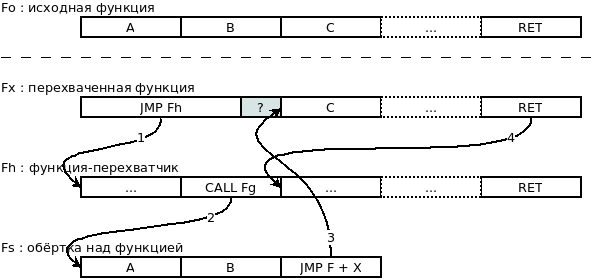
\includegraphics[width=\textwidth]{img/hookScheme}
  \caption{Процесс перехвата функции}
\end{figure}

На рисунке 1, цифрой 1 отмечена передача управления от целевой функции к функции-перехватчику (команда JMP), цифрой 2 — вызов оригинальной функции с использованием сохранённой части пролога (команда CALL), цифрой 3 — возврат управления к части оригинальной функции, не подвергавшейся изменению (команда JMP), и, наконец, цифрой 4 — возврат управления по завершению вызова оригинальной функции из перехватчика (команда RET). Таким образом, обеспечивается возможность использования реализуемых перехватываемой функцией возможностей.
\subsubsection{Реализация перехвата функций}
Будем описывать каждую перехватываемую функцию следующей структурой:
\lstinputlisting[caption=Структура функции для перехвата, language={}]{sourceCode/hook/habr/lst4.txt}
\begin{itemize}
\item \textbf{name} — имя перехватываемой функции (имя символа);
\item \textbf{length} — длина затираемой последовательности инструкций пролога;
\item \textbf{handler} — адрес функции-перехватчика;
\item \textbf{target} — адрес самой целевой функции;
\item \textbf{target\_map} — адрес доступной для записи проекции целевой функции;
\item \textbf{origin} — адрес функции-переходника, используемой для доступа к исходной функциональности;
\item \textbf{origin\_map} — адрес доступной для записи проекции соответствующего переходника;
\item \textbf{usage} — счётчик «залипаний», учитывающий число спящих в перехвате потоков.
\end{itemize}
Каждая перехватываемая функция должна быть представлена такой структурой. Для этого, дабы упростить регистрацию перехватчиков, используется макрос DECLARE\_KHOOK(...), представляемый следующим образом:
\lstinputlisting[caption=Макрос регистрации перехватчика, language={}]{sourceCode/hook/habr/lst5.txt}

Вспомогательные макросы \_\_DECLARE\_TARGET\_ALIAS(...), \_\_DECLARE\_TARGET\_ORIGIN(...) декларируют перехватчик и переходник (32 nop'а). Саму структуру объявляет макрос \_\_DECLARE\_TARGET\_STRUCT(...), посредством атрибута section определяя её в специальную секцию (.khook).

При загрузке модуля ядра происходит перечисление всех зарегистрированных перехватов (khook\_for\_each), представленных структурами в секции с именем .khook. Для каждого из них осуществляется поиск адреса соответствующего символа (get\_symbol \_address), а также настройка вспомогательных элементов, включая создание отображений (map\_witable):
\lstinputlisting[caption=Загрузка модуля, language={}]{sourceCode/hook/habr/lst6.txt}
Важную роль играет функция init\_origin\_stub, осуществляющая инициализацию и построение переходника, используемого для вызова оригинальной функции после перехвата:
\lstinputlisting[caption=Переходник для вызова оригинальной функции, language={}]{sourceCode/hook/habr/lst7.txt}
Как видно, для определения количества затираемых при патчинге пролога инструкций используется дизассемблер udis86. В принципе, для этой цели подойдёт любой дизассемблер с функцией определения длины инструкции (т.н. Length-Disassembler Engine, LDE). Для этих целей используется полноценный дизассемблер udis86, который имеет BSD-лицензию и хорошо зарекомендовал себя. Как только число инструкций определено, происходит их копирование по адресу origin\_map, что соответствует RW-проекции 32-байтного переходника origin. В завершении, после сохранённых команд с использованием x86\_put\_jmp вставляется команда, возвращающая управление на оригинальной код целевой функции, не подвергшийся изменению.

Последним элементом, позволяющим сделать модификацию кода ядра безопасной, является механизм stop\_machine:
\lstinputlisting[caption=Механизм безопасной модификации ядра, language={}]{sourceCode/hook/habr/lst8.txt}
Суть в том, что stop\_machine осуществляет выполнение функции fn с заданным набором активных в момент выполнения процессоров, что задаётся соответствующей маской cpumask. Именно это позволяет использовать данный механизм для осуществления модификации кода ядра, т.к. задание соответствующей маски автоматически исключает необходимость отслеживания тех потоков ядра, выполнение которых может затрагивать модифицируемый код.

Далее, по ходу работы, с помощью макроса \textbf{DECLARE\_KHOOK} будут написаны перехватчики заданных функций.



\section{Системная функция fork}
\textbf{fork()}\cite{fork} - системный вызов, создающий новый процесс (потомок), который является практически полной копией процесса-родителя, выполняющего этот вызов. Дочерний и родительский процессы находятся в отдельных пространствах памяти.  Создавшийся процесс будет занят выполнением того же кода ровно с той же точки, что и исходный процесс.\\
\textbf{Расположение: }.../kernel/fork.c\\
\textbf{Синтаксис: }long sys\_fork(struct pt\_regs *regs)\\\\
В виде параметра выступает указатель на структуру с регистрами, возращаемое значение - id процесса потомка.\\\\
В ходе экспериментов выяснилось, что вместо fork() вызывается функция \textbf{clone()}.\\
\textbf{clone()}\cite{clone} - создаёт новый процесс подобно fork. Но в отличие от fork(), clone() позволяет процессу-потомку использовать некоторые части контекста выполнения совместно с вызывающим процессом, например: область памяти, таблица файловых дескрипторов и таблица обработчиков сигналов.\\
\textbf{Расположение: }.../arch/x86/kernel/process\_64.c\\
\textbf{Синтаксис: }long sys\_clone(unsigned long clone\_flags, unsigned long newsp, void \_\_user *parent\_tid, void \_\_user *child\_tid, struct pt\_regs *regs)\\
\textbf{Аргументы конструктора}:
\begin{enumerate}
\item clone\_flags - параметры копирования(что копировать, а что нет). 
\item newsp - новый адрес функции;
\item parent\_tid и child\_tid - два указателя в пространстве пользователя, для хренения id родительского и дочернего процессов;
\item regs - структура регистрова процесса родителя.
\end{enumerate}

\subsection{Программы для анализа}
Запуск программы произведен на версии ядра 4.13.\\
Представленные программы написаны на языке \textbf{C}, и показывают использование заданной функции на пользовательском уровне.
\subsubsection{Программа с использованием fork}
Программа, с помощью функции fork() создает процесс-потомок.
\lstinputlisting[caption=forkExample.c, language=C, label={lst:fork1}]{sourceCode/fork/programs/forkExample.c}
Программа выводит информацию о каждом процессе.
\lstinputlisting[caption=forkExample.log]{sourceCode/fork/kernel_4.13/forkExample.log}
\subsubsection{Программа с использованием clone}
Программа, с помощью функции clone() создает процесс-потомок.
\lstinputlisting[caption=cloneExample.c, language=C]{sourceCode/fork/programs/cloneExample.c}
Каждый процесс выводит в консоль значения от 0 до 9.
\lstinputlisting[caption=cloneExample.log, language=C, label={lst:clone1}]{sourceCode/fork/kernel_4.13/cloneExample.log}
\subsubsection{Программа с прямым вызовом fork}
Программа напрямую вызывает системную функцию fork(), по её номеру(57), записанному в таблице системных функций. Таким образом игнорируется обвязка glibc.
\lstinputlisting[caption=fork2.c, language=C, label={lst:fork2}]{sourceCode/fork/programs/fork2.c}
\lstinputlisting[caption=fork2.log]{sourceCode/fork/kernel_4.13/fork2.log}

\subsection{Ядро версии 4.13.0-38-generic}
\subsubsection{Анализ strace}
С помощью команды \textbf{strace} посмотрим лог вызовов для программы fork() приведенной в листинге \ref{lst:fork1}.
\lstinputlisting[firstnumber=1,firstline=1,lastline=28, caption=forkStrace.log]{sourceCode/fork/kernel_4.13/forkStrace.log}
По части лога видно, что сперва происходит отображение в память, а затем и создание нового процесса. Однако создание нового процесса было произведено с помощью системной функции clone(), а не fork().

Дополнительно посмотрим лог вызовов программы с clone() (листинг \ref{lst:clone1}).
\lstinputlisting[firstnumber=1,firstline=1,lastline=28, caption=cloneStrace.log]{sourceCode/fork/kernel_4.13/cloneStrace.log}


Как видно из логов, для fork() и clone() был использован именно системный вызов clone(). Это связано с тем, как \textbf{glibc} интерпретирует эти команды. 

Теперь рассмотрим историю вызовов с прямым вызовом fork() по его номеру (программа из листинга \ref{lst:fork2}).
\lstinputlisting[firstnumber=1,firstline=1,lastline=38, caption=fork2Strace.log, label={lst:trueFork}]{sourceCode/fork/kernel_4.13/fork2Strace.log}
Как видно, в строчке 32 была вызвана системная функция fork(), которая вернула значение 7724 (pid процесса потомка).

\subsubsection{Анализ glibc}

Проанализируем исходный код glibc, в данном случае программы компилировались используя \textbf{glibc 2.23}. Исходный код, различных версий доступен по ссылке\cite{glibc}.

По пути \textbf{glibc\_2.23/sysdeps/nptl/fork.c} имеется файл fork.c, в котором в строках 124-129 и представлен вызов функции.
\lstinputlisting[firstnumber=124,firstline=124,lastline=129, caption=glibc\_2.23/sysdeps/nptl/fork.c]{sourceCode/fork/glibc/2.23/sysdeps/nptl/fork.c}
Реализация макроса представлена по пути \textbf{glibc\_2.23/sysdeps/unix/sysv/linux/x86\_64/arch-fork.h} в файле arch-fork.h.
\lstinputlisting[firstnumber=24,firstline=24,lastline=27, caption=glibc\_2.23/sysdeps/unix/sysv/linux/x86\_64/arch-fork.h]{sourceCode/fork/glibc/2.23/sysdeps/unix/sysv/linux/x86_64/arch-fork.h}

Как видно из реализации макроса, вызывается системный вызов clone(), а не fork().

Дополнительно рассмотрим исходный код glibc версии 2.15.90.

По пути \textbf{glibc\_2.15/nptl/sysdeps/unix/sysv/linux/} имеется файл fork.c, в котором в строках 129-134 представлен вызов функции.

\lstinputlisting[firstnumber=129,firstline=129,lastline=134, caption=glibc\_2.15/nptl/sysdeps/unix/sysv/linux/fork.c]{sourceCode/fork/glibc/2.15/nptl/sysdeps/unix/sysv/linux/fork.c}

Реализация макроса представлена по пути \textbf{glibc\_2.15/nptl/sysdeps/unix/sysv/linux/x86\_64/} в файле fork.c.

\lstinputlisting[firstnumber=25,firstline=25,lastline=28, caption=glibc\_2.15/nptl/sysdeps/unix/sysv/linux/x86\_64/fork.c]{sourceCode/fork/glibc/2.15/nptl/sysdeps/unix/sysv/linux/x86_64/fork.c}



Версия 2.15 имеет уже 6 летнюю давность, и в ней также вызывался системный вызов clone(). Единственным отличием оказалось различное расположение файлов, с исходным кодом. 

Если изучить прототипы fork() и clone(), то можно прийти к выводу что использование clone() началось для общего облегчения процессов в Linux системах, так как используя clone(), имеется возможность разделения между процессами:
\begin{itemize}
\item контекста;
\item памяти;
\item файловых дескрипторов;
\item обработчиков сигналов.
\end{itemize}
Все это приводит к более гибкому созданию нового процесса, что fork() не позволяет.


Конечно можно более подробно проанализировать хронологию, но не не стоит отклоняться от основной темы данной работы.
\subsubsection{Анализ исходного кода}
Рассмотрим часть файла \textbf{syscall\_64.tbl}, именно в данном файле определены системные вызовы.
\lstinputlisting[firstnumber=63,firstline=63,lastline=69, caption=.../arch/x86/syscalls/syscall\_64.tbl, label={lst:64tbl}]{sourceCode/kernel/4.13/arch/x86/entry/syscalls/syscall_64.tbl}
В строчке 65 для вызова clone() присвоен номер 56, а для fork() 57. Именно благодарю этому уникальному номеру, ранее удалось вызвать системный вызов напрямую.

Для различных архитектур, номера системных вызовов могут несколько отличаться.

Далее рассмотрим заголовочный файл \textbf{syscalls.h}.
\lstinputlisting[firstnumber=837,firstline=837,lastline=848, caption=.../include/linux/syscalls.h]{sourceCode/kernel/4.13/include/linux/syscalls.h}
В данном файле определены прототипы объявленных в таблице системных вызовов. Как минимум каждая из платформ должна реализовывать все объявленные параметры в прототипе, но также может и расширять их, при необходимости.

Исходный код(основная часть), находится в файле \textbf{fork.c}, по пути \textbf{/kernel}. Ввиду обилия кода(2467 строк), файл приложен к отчету, а далее представлено пояснение основных моментов.

Начало реализация представлено в строке 2006.
\lstinputlisting[firstnumber=2006,firstline=2006,lastline=2036, caption=.../kernel/fork.c]{sourceCode/kernel/4.13/kernel/fork.c}
Аргументы функции:
\begin{enumerate}
\item \textbf{clone\_flags} - флаг, для определения того, что именно нужно копировать;
\item \textbf{parent\_tid и child\_tid} - два указателя в пространстве пользователя, для хренения id родительского и дочернего процессов;
\item \textbf{stack\_start} - адрес начала стека с процессами;
\item \textbf{tls} - определение локального хранилища для нового процесса
\end{enumerate}
\begin{figure}[H]
  \centering
  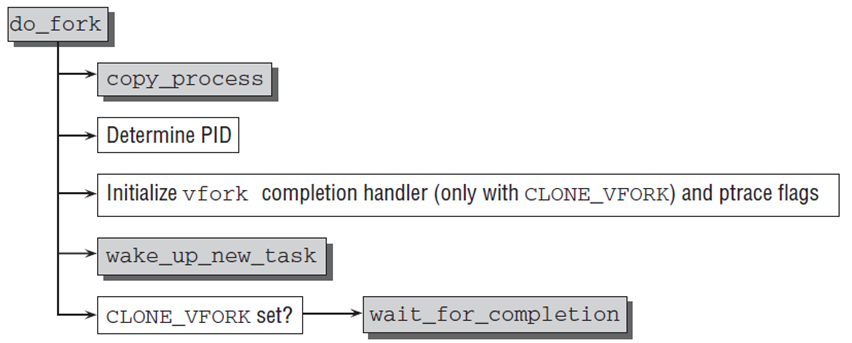
\includegraphics[width=\textwidth]{img/do_fork}
  \caption{Схема работы do\_fork}
\end{figure}
Основным действием является вызов функции \textbf{(copy\_process)}.

\begin{figure}[H]
  \centering
  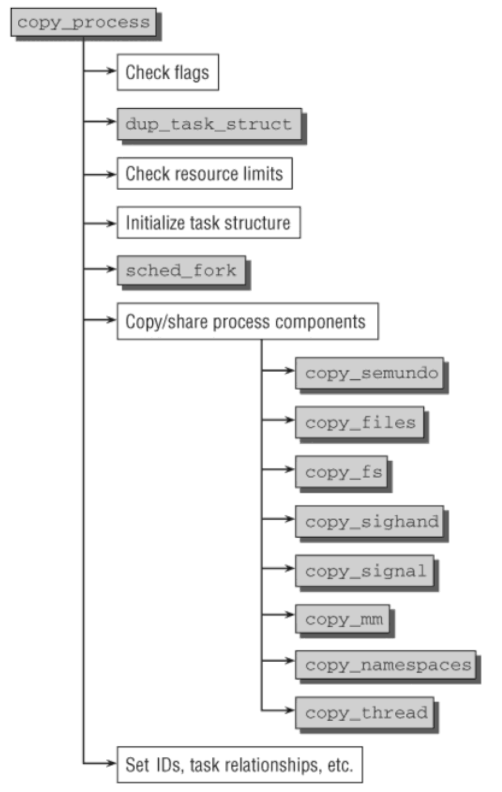
\includegraphics[width=.7\textwidth]{img/copy_process}
  \caption{Схема работы copy\_process}
\end{figure}
\textbf{copy\_process()}, также как и do\_fork(), начинает свою работу спроверки на сочетание установленных флагов. Опишем некоторые проверки:
\begin{itemize}
\item если установлен флаг CLONE\_THREAD, но не установлен флаг CLONE\_SIGHAND, то возвращается ошибка, так как потоки группыдолжны разделять сигналы;
\item если установлен флаг CLONE\_SIGHAND, но не установлен флаг CLONE\_VM, то возвращается ошибка, так как общие обработчикисигналов, подразумевают общее адресное пространство.
\end{itemize}
Далее вызывается функция dup\_task\_struct() (определена в файле kernel/fork.c), которая создает новый экземпляр структуры task\_struct и копирует в него различные дескрипторы, относящиеся к текущему процессу. Затем в copy\_process производится проверка лимитов и полномочий, производится проверка на "fork bomb"\cite{forkBomb}.

Выполняются вспомогательные действия, включающие инициализацию различных полейструктуры task\_struct. Потом происходит вызов функций, выполняющих копирование составляющих процесса: 
\begin{itemize}
\item таблицы дескрипторов открытых файлов (copy\_files);
\item таблицы сигналов и обработчиков сигналов(copy\_signal и copy\_sighand);
\item адресного пространства процесса(copy\_mm) и структуры thread\_info (copy\_thread).
\end{itemize}
Затем только что созданная задача назначается процессору из числа разрешенных для ее выполнения (cpus\_allowed). После того как новый процесс унаследует приоритет родительского процесса, выполняется еще небольшое число вспомогательных действий и происходит возврат в do\_fork().


По завершению \textbf{copy\_process}, инициализируется обработчики для \textbf{vfork}(если флаг был передан). Далее идет вызов \textbf{wake\_up\_new\_task}(помещает новый процесс в очередь выполненияи инициирует его выполнение), что является стандартным для всех новых процессов. И наконец, есть выставлен флаг на vfork, необходимо дождаться его завершения, прежде снова передать управление родительскому процессу.


\subsection{Ядро версии 2.6.32-21-generic}
\subsubsection{Анализ strace}
Ввиду полного совпадения(анализируемой функции) логов, по сравнению с логами ядра версии 4.13, их рассмотрение не требуется. Но они также приложены к данной работе.

\subsubsection{Анализ исходного кода}
Реализация также представлена в файле \textbf{fork.c}, по пути \textbf{/kernel/fork.c}.

Начало реализация представлено в строке 1166.
\lstinputlisting[firstnumber=1166,firstline=1166,lastline=1183, caption=.../kernel/fork.c]{sourceCode/kernel/2.6.32/kernel/fork.c}
Вся реализация уже описана для версии ядра 4.13, рассмотрим отличия:
\begin{enumerate}
\item у конструктора функции убран аргумент \textbf{tls} (определение локального хранилища);
\item убраны различные проверки флагов, которые ранее информировали \textbf{ptrace} о вызванном событии.
\end{enumerate}
В остальном, за исключением меньшего количество проверок входных данных, все идентично.

\subsection{Перехват вызова}
Для ядра версии 4.13 компиляция не удалась(что вполне ожидаемо), так как используемые функции и символы были убраны из экпорта ядра, то есть получить к ним доступа более не предоставляется возможным.

Как вариант, на новых версиях ядер, для перехвата можно использовать \textbf{LSM}(Linux Security Modules), но в моем случаем не все системные вызовы им поддерживаются. Поэтому, перехват вызовов будет предстален для версии ядра \textbf{2.6.32-21}.

В файле по пути \textbf{/include/asm-generic/} имеется файл \textbf{syscalls.h}, в котором определен прототип fork().
\lstinputlisting[firstnumber=17,firstline=17,lastline=19, caption=.../kernel/asm-generic/syscalls.h]{sourceCode/kernel/2.6.32/asm-generic/syscalls.h}

Для того, чтобы перехватить данную функцию, напишем метод khook\_sys\_fork, который будет перехватывать системный вызов и перенаправлять управление нам:

\lstinputlisting[firstnumber=203,firstline=203,lastline=217, caption=Функция перехвата fork()]{sourceCode/fork/hookProgram/module-init.c}

Полный код программы приведен в приложении.  

Для компиляции модуля ядра, необходим специальный Makefile.
\lstinputlisting[caption=Makefile]{sourceCode/fork/hookProgram/Makefile}
Выполним Makefile для компиляции модуля ядра:
\lstinputlisting[caption=Лог сборки]{sourceCode/fork/hookProgram.logs/make.log}
Далее встроим модуль в ядро:
\lstinputlisting[firstnumber=1,firstline=1,lastline=1, caption=Встраивание модуля в ядро]{sourceCode/fork/hookProgram.logs/insrm.log}
Далее, в другом окне терминала выполним программу с прямым вызовом fork, и посмотрим системный лог.
\lstinputlisting[caption=Лог с сообщением о перехвате]{sourceCode/fork/hookProgram.logs/hook.log}
Как видно из лога, перехват не повлиял на работоспособность функции, а в системный лог, как и ожидлось было добавлено сообщение о перехвате. 

Теперь выгружаем модуль из ядра.
\lstinputlisting[firstnumber=1,firstline=2,lastline=2, caption=Выгрузка модуля из ядра]{sourceCode/fork/hookProgram.logs/insrm.log}
После выгрузки, перехватчик более не активен.



\subsection{Общая иерархия вызовов}
Дополнительно, если привести иерархию вызовов, то можно заметить что не только fork() и clone() используют функцию do\_fork().
\begin{figure}[H]
  \centering
  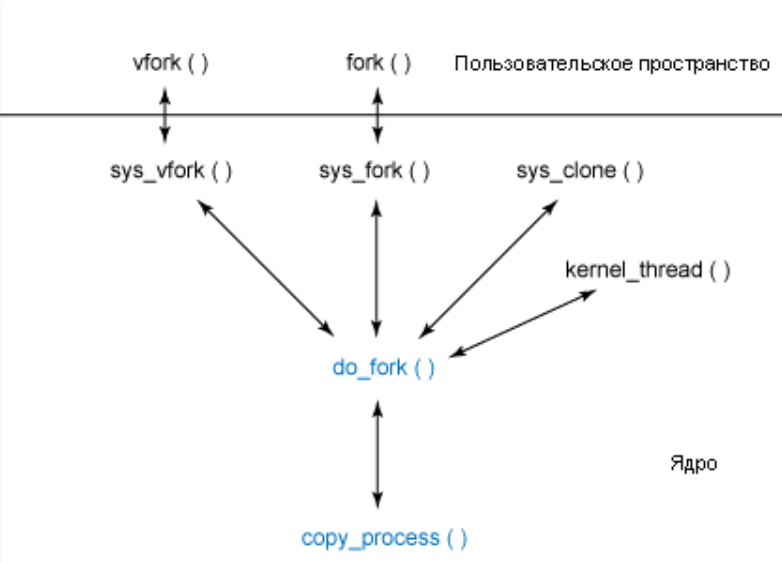
\includegraphics[width=.65\textwidth]{img/hierarchy}
  \caption{Иерархия вызовов при создании процесса}
\end{figure}


\section{Системная функция execve}
\textbf{execve()}\cite{execve} - выполняет программу, задаваемую аргументом filename.\\
\textbf{Расположение: }.../fs/exec.c\\
\textbf{Синтаксис: } long sys\_execve(char \_\_user *filename, char \_\_user * \_\_user *argv, char \_\_user * \_\_user *envp, struct pt\_regs *regs)\\
Аргементы:
\begin{itemize}
\item \textbf{filename} - имя файла для выполнения;
\item \textbf{argv и envp} - вектор аргументов и среда выполнения;
\item \textbf{regs} - указатель на структуру регистров, на момент вызова данной функции.
\end{itemize}
\subsection{Программы для анализа}
Запуск программы произведен на версии ядра 4.13.\\

Программа печатает в консоль сообщение, часть которого передается в виде одно из аргументов запуска. Также, в цикле выводятся все переменные окружения. Для определения размера массива с переменными, согласно документации, последний элемент будет NULL.
\lstinputlisting[caption=sys\_execve.c, label={lst:execve}]{sourceCode/execve/programs/sys_execve.c}
\lstinputlisting[caption=sys\_execve.log]{sourceCode/execve/kernels/4.13/sys_execve.log}
Из лога можно видеть множество системных констант, можно определить в каком каталоге был запуск, каким пользователем, на какой системе и многое другое.
\subsection{Ядро версии 4.13.0-38-generic}
\subsubsection{Анализ strace}
Для сокращения лога, приведены первые 2 строчки лога strace.
\lstinputlisting[firstnumber=1,firstline=1,lastline=2, caption=sys\_execve\_strace.log]{sourceCode/execve/kernels/4.13/sys_execve_strace.log}
Аргументы соответствуют ожиданиям, первый аргумент соответствует программе для запуска. Далее расположен массив аргументов, передаваемых в запускаемую программу. И наконец передаются переменные окружения, правда в данном случае, из-за их обилия они скрыты, и показано лишь их количество.
\subsubsection{Анализ исходного кода}
Основная часть, архитектурно независимого кода находится в файле \textbf{exec.c} по пути \textbf{/fs/}.
\lstinputlisting[firstnumber=1828,firstline=1828,lastline=1835, caption=../fs/exec.c]{sourceCode/kernel/4.13/fs/exec.c}
Если сравнивать с ядром керсии 2.6.32, то в данном случае, оригинальная функция \textbf{do\_execve} превратилась в некоторую обертку, а основная функциональность была перенесена в функцию \textbf{do\_execveat\_common}.
\lstinputlisting[firstnumber=1679,firstline=1679,lastline=1686, caption=../fs/exec.c]{sourceCode/kernel/4.13/fs/exec.c}
Принцип работы представлен на схеме далее.
\begin{figure}[H]
  \centering
  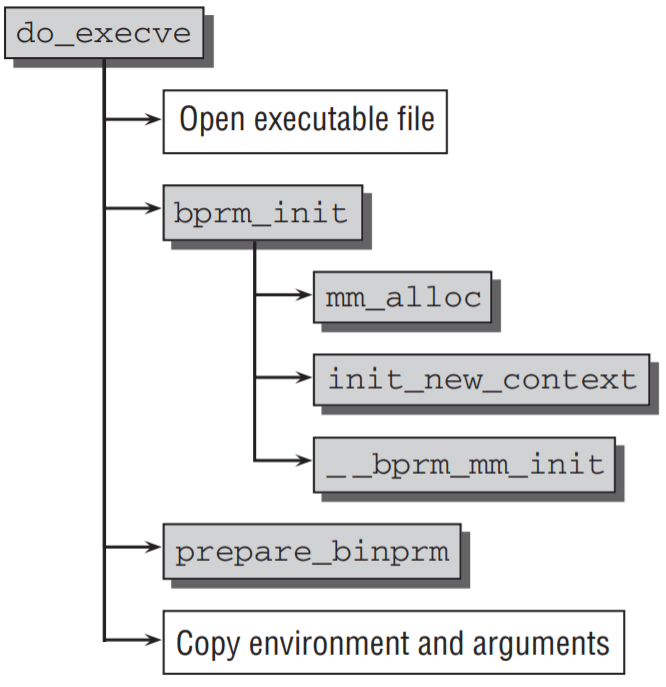
\includegraphics[width=.6\textwidth]{img/do_execve}
  \caption{Схема работы do\_execve}
\end{figure}
\begin{enumerate}
\item Различные проверки корректности аргументов, открытие перадаваемого файла, получение его дескриптора;
\item Вызов функции \textbf{bprm\_init}
\begin{enumerate}
\item \textbf{mm\_alloc} - генерация структуры \textbf{mm\_struct}, для организации адресного пространства процесса;
\item \textbf{init\_new\_context} - создание нового контекста для процесса;
\item \textbf{\_\_bprm\_mm\_init} - установка нового процесса в стек;
\end{enumerate}
\item \textbf{prepare\_binprm} - предоставления доступа к различным значениям(euid, egid, имя файла, окружение ...) родительского процесса(ов).
\end{enumerate}

\subsection{Ядро версии 2.6.32-21-generic}
\subsubsection{Анализ strace}
Лог strace неотличается от версии ядра 4.13, за исключением того что, в массиве переменных окружения было передано 38 переменных вместо 60. Более подробно можно посмотреть в приложенных логах к данной работе.
\subsubsection{Анализ исходного кода}
Основная часть, архитектурно независимого кода находится в файле \textbf{exec.c} по пути \textbf{/fs/}.
\lstinputlisting[firstnumber=1069,firstline=1069,lastline=1076, caption=../fs/exec.c]{sourceCode/kernel/2.6.32/fs/exec.c}
В отличии от ядра 4.13, в данном случае никакой обертки над функцией нет. По коду, основным отличием является то, что отдельные функции из \textbf{bprm\_init} были перенесены непосредственно в тело функции \textbf{do\_execve}.

\subsection{Перехват вызова}
В файле по пути \textbf{/include/asm-generic/} имеется файл \textbf{syscalls.h}, в котором определен прототип execve().
\lstinputlisting[firstnumber=25,firstline=25,lastline=28, caption=.../kernel/asm-generic/syscalls.h]{sourceCode/kernel/2.6.32/asm-generic/syscalls.h}
Для того, чтобы перехватить данную функцию, напишем метод khook\_sys\_execve, который будет перехватывать системный вызов и перенаправлять управление нам:
\lstinputlisting[firstnumber=203,firstline=203,lastline=222, caption=Функция перехвата execve()]{sourceCode/execve/hookProgram/module-init.c}

Помимо сообщения о перехвате, выводим название программы, запуск которой был произведен. Полный код программы приведен в приложении.  

Выполним Makefile для компиляции модуля ядра:
\lstinputlisting[firstnumber=1,firstline=1,lastline=9, caption=Лог сборки]{sourceCode/execve/hookProgram.logs/make.log}
Далее встроим модуль в ядро:
\lstinputlisting[firstnumber=1,firstline=10,lastline=10, caption=Лог сборки]{sourceCode/execve/hookProgram.logs/make.log}
Далее, в другом окне терминала выполним программу, представленную в листинге \ref{lst:execve}, и посмотрим системный лог.
\lstinputlisting[caption=Системный лог]{sourceCode/execve/hookProgram.logs/kern.log}
Как видно из лога, функция была успешно перехвачена, было выведено соответствующее сообщение и имя файла для запуска, в данном случае \textbf{./sys\_execve.o}.

Теперь выгружаем модуль из ядра.
\lstinputlisting[firstnumber=1,firstline=11,lastline=11, caption=Выгрузка модуля из ядра]{sourceCode/execve/hookProgram.logs/make.log}
После выгрузки, перехватчик более не активен.


\section{Системная функция exit}
\textbf{exit()}\cite{exit} - завершает работу программы. Все дескрипторы файлов, принадлежащие процессу, закрываются; все его дочерние процессы начинают управляться процессом 1 (init), а родительскому процессу посылается сигнал SIGCHLD.\\
\textbf{Расположение: }.../kernel/exit.c\\
\textbf{Синтаксис: } long sys\_exit(int error\_code)\\
Аргементы:
\begin{itemize}
\item \textbf{error\_code} - код выхода.
\end{itemize}

\subsection{Программы для анализа}
Запуск программы произведен на версии ядра 4.13.\\

Программа выводит в консоль два сообщения, одно до, а другое после системного вызова exit, по коду 60 (системный номер функции, взят из листинга \ref{lst:64tbl}).
\lstinputlisting[caption=sys\_exit.c, label={lst:exit}]{sourceCode/exit/programs/sys_exit.c}
\lstinputlisting[caption=sys\_exit.log]{sourceCode/exit/kernels/4.13/sys_exit.log}
Как и ожидалось, после системного вызова exit, никаких сообщений выведено не было.

\subsection{Ядро версии 4.13.0-38-generic}
\subsubsection{Анализ strace}
\lstinputlisting[caption=sys\_exit\_strace.log]{sourceCode/exit/kernels/4.13/sys_exit_strace.log}
Внимания стоит уделить строчкам 30 и 32. В строчке 30 происходит вывод текста в консоль, а далее, в строке 32 происходит вызов систеного вызова exit, после которого, никаких других сисмных вызовов не последовало.
\subsubsection{Анализ исходного кода}
Основная часть, архитектурно независимого кода находится в файле \textbf{exit.c} по пути \textbf{/kernel/}. Далее приведено лишь начало функции \textbf{do\_exit}.
\lstinputlisting[firstnumber=763,firstline=763,lastline=777, caption=../kernel/exit.c]{sourceCode/kernel/4.13/kernel/exit.c}
По ходу выполнения производятся следующие действия:
\begin{enumerate}
\item В вызвавшем процессе закрываются все дескрипторы открытых файлов;
\item Если родительский процесс находится в состоянии вызова wait, то системный вызов wait завершается, выдавая родительскому процессу в качестве результата идентификатор терминировавшегося процесса;
\item Если родительский процесс не находится в состоянии вызова wait, то процесс, вызвавший exit, переходит в состояние зомби. Это такое состояние, когда процесс занимает только элемент в таблице процессов и не занимает памяти ни в адресном пространстве пользователя, ни в адресном пространстве ядра. Элемент таблицы процессов, занятый зомби-процессом, содержит информацию о времени, затраченном процессом.
\end{enumerate}
У всех существующих потомков терминировавшихся процессов, а также у зомби-процессов идентификатор родительского процесса устанавливается равным 1. Таким образом, все эти процессы наследуются инициализационным процессом.

Все присоединенные разделяемые сегменты памяти отсоединяются и в связанных с ними структурах данных значения полей shm\_nattach уменьшаются на 1.

Родительскому процессу посылается сигнал SIGCLD (завершение порожденного процесса).

\subsection{Ядро версии 2.6.32-21-generic}
\subsubsection{Анализ strace}
Лог strace неотличается от версии ядра 4.13. Лог приложен к работе.
\subsubsection{Анализ исходного кода}
Как и у ядра 4.13, основная часть кода расположена в файле \textbf{exit.c}, а далее приведено начало функции \textbf{do\_exit}.
\lstinputlisting[firstnumber=796,firstline=796,lastline=809, caption=../kernel/exit.c]{sourceCode/kernel/2.6.32/kernel/exit.c}
Вся реализация, подобна реализации в ядре 4.13, за исключением того, что в данном случае, порядок действий в несколько ином порядке, а также уменьшено количество действий по обеспечению откладочной информации, например отсутствует нотификация ptrace.

\subsection{Перехват вызова}
В файле по пути \textbf{/include/linux/} имеется файл \textbf{syscalls.h}, в котором определен прототип exit().
\lstinputlisting[firstnumber=418,firstline=418,lastline=418, caption=.../kernel/linux/syscalls.h]{sourceCode/kernel/2.6.32/linux/syscalls.h}
Для того, чтобы перехватить данную функцию, напишем метод khook\_sys\_exit, который будет перехватывать системный вызов и перенаправлять управление нам:
\lstinputlisting[firstnumber=203,firstline=203,lastline=218, caption=Функция перехвата exit()]{sourceCode/exit/hookProgram/module-init.c}

При успешном перехвате, в системный лог добавляется запись о успешном перехвате.

Выполним Makefile для компиляции модуля ядра:
\lstinputlisting[firstnumber=1,firstline=1,lastline=10, caption=Лог сборки]{sourceCode/exit/hookProgram.logs/make.log}
Далее встроим модуль в ядро:
\lstinputlisting[firstnumber=1,firstline=11,lastline=11, caption=Лог сборки]{sourceCode/exit/hookProgram.logs/make.log}
Далее, в другом окне терминала выполним программу, представленную в листинге \ref{lst:exit}, и посмотрим системный лог.
\lstinputlisting[caption=Системный лог]{sourceCode/exit/hookProgram.logs/kern.log}
Как видно из лога, функция была успешно перехвачена.

Теперь выгружаем модуль из ядра.
\lstinputlisting[firstnumber=1,firstline=13,lastline=13, caption=Выгрузка модуля из ядра]{sourceCode/exit/hookProgram.logs/make.log}
После выгрузки, перехватчик более не активен.\\\\
\textbf{Примечание:} после попытки выгрузки модуля, консоль в которой производилась работа перестает отвечать на команды, а через некоторое время и сама система зависает.

\section{Модификация системных вызовов}
Модификации будут применены относительно исходного кода ядра версии 4.13.0.
\subsection{Вносимые модификации}
В виде примера модификации, будет производится запись сообщения о вызове функции в системный лог. А для \textbf{execve} также вывод имени запускаемого файла.
\subsubsection{Системная функция fork}
В начале основной функции \textbf{do\_fork}(файл \textbf{/kernel/fork.c}) было добавлено информационное сообщение(строка 2016) для записи в системный лог.
\lstinputlisting[firstnumber=2006,firstline=2006,lastline=2017, caption=Модифицированный fork]{sourceCode/modification/modifiedUtils/fork.c}

\subsubsection{Системная функция execve}
Модификации подверглась функция \textbf{do\_execveat\_common} из файла \textbf{/fs/exec.c}. 
\lstinputlisting[firstnumber=1682,firstline=1682,lastline=1696, caption=Модифицированный exec]{sourceCode/modification/modifiedUtils/exec.c}
Сразу после успешной проверки на валидность файла(строка 1693), происходит вывод информационного сообщения(строка 1696).
\subsubsection{Системная функция exit}
В начале основной функции \textbf{do\_exit}(файл \textbf{/kernel/exit.c}) было добавлено информационное сообщение(строка 765) для записи в системный лог.
\lstinputlisting[firstnumber=763,firstline=763,lastline=765, caption=Модифицированный exit]{sourceCode/modification/modifiedUtils/exit.c}


\subsection{Перекомпиляция ядра}
Для начала необходимо скачать исходный код интересующей версии ядра, в данном случае это также ядро 4.13.0.

Далее необходимо установить некоторые пакеты следующей командой:
\lstinputlisting[caption=Установка недостающий пакетов]{sourceCode/modification/guide/install_1.log}

Архив с исходным кодом был распакован по пути \textbf{/usr/src/}. Перейдем в эту папку и выполним команду:
\lstinputlisting[caption=Конфигурация ядра]{sourceCode/modification/guide/install_2.log}
После выполнения данной команды, в консоли откроется меню для конфигруации ядра.

\begin{figure}[H]
  \centering
  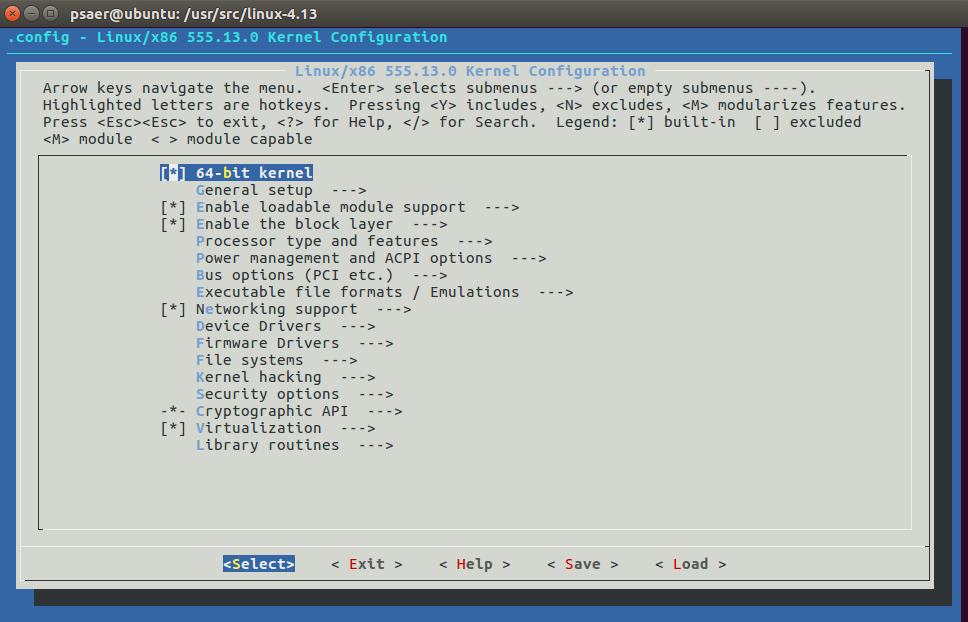
\includegraphics[width=\textwidth]{img/menuconfig}
  \caption{Конфигурация ядра}
\end{figure}

В данном случае, в нем нет необходимости, закрываем его.

Перед компиляцией ядра, внесем изменения в файл \textbf{Makefile}, который находится в корне разархивированного ядра.
\lstinputlisting[firstnumber=1,firstline=1,lastline=5,caption=Файл Makefile]{sourceCode/modification/Makefile.txt}
В представленных первых 5 строках представлена основная информация о версии ядра. В моем случае, вместо версии 4 была поставлена версия 555.\\\\

Теперь приступаем к компиляции, для этого выполняем следующую команду:
\lstinputlisting[caption=Компиляция ядра]{sourceCode/modification/guide/install_3.log}
Ключ \textbf{j} означает количество задействованных ядер системы. В моем случае, в настройках VMware, виртуальной машине было выделено 3 ядра процессора.

Первые две команды, из листинга выше, выполняют компиляцию ядра, а последняя компилирует въедино в образ ядра системы.

Процесс, в моем случае занимиает около 20 минут.\\\\
Далее необходимо включить показ меню \textbf{GRUB}. Для этого редактируем файл \textbf{grub} по пути \textbf{/etc/default/}.
\lstinputlisting[caption=Файл grub]{sourceCode/modification/grub.txt}
В данном файле необходимо закомментировать(поставить знак \# в начале строки) строки 7 и 8.

После этого перезагружаем систему. 

После старта виртуальной машины, будет показано меню GRUB.

\begin{figure}[H]
  \centering
  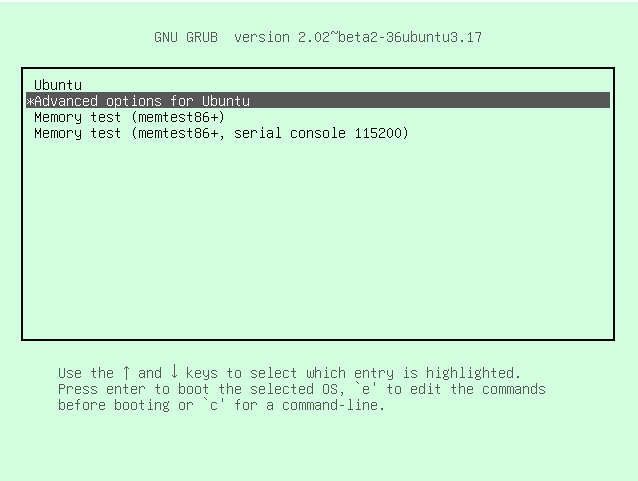
\includegraphics[width=.8\textwidth]{img/grub_1}
  \caption{Меню GRUB}
\end{figure}

Выбираем пункт \textbf{Advance options for Ubuntu} и нажимаем enter. Будет выведен список с воможными ядрами для загрузки.

\begin{figure}[H]
  \centering
  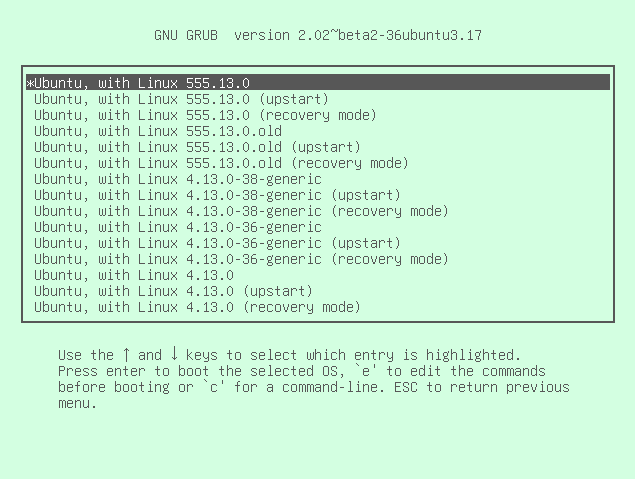
\includegraphics[width=.8\textwidth]{img/grub_2}
  \caption{Выбор ядра в GRUB}
\end{figure}
Выбираем скомпилированное ядра версии 555.13.0. В случае корректно скомпилированного ядра, система успешно загрузится.

Дополнительно, после загрузки ОС, можно проверить версию ядра.
\lstinputlisting[caption=Версия ядра]{sourceCode/modification/uname.txt}
Теперь можно приступить к тестированию.

\subsection{Проверка модификации}

Выполним программу из листинга \ref{lst:fork2}.
\lstinputlisting[caption=Выполнением программы с прямым вызовом fork]{sourceCode/modification/check/fork.log}

Для поиска сообщений, которые записываются в системный лог, будет использована следующая команда:
\lstinputlisting[firstnumber=1,firstline=1,lastline=1,caption=Команда для поиска некоторого сообщения]{sourceCode/modification/check/fork.txt}
Поиск происходит рекурсивно, в каталоге \textbf{/var/log/} на предмет наличия в тексте \textbf{fork}.

\lstinputlisting[firstnumber=122,firstline=122,lastline=130,caption=Результаты поиска fork]{sourceCode/modification/check/fork.txt}
Ввиду обилия вывода, приведена лишь часть, из которой видно:
\begin{enumerate}
\item Системный вызов \textbf{fork} успешно произовит записи в системный лог, причем, судя по логу, он был вызван системой при загрузки множество раз;
\item В строчке 127, была обнаружена запись от модифицированного вызова \textbf{exec};
\item В строчке 130, была обнаружена запись о ранее вводимой команде, то есть в систему встроен некоторый логгер пользовательских команд.
\end{enumerate}
Теперь проверим модификацию вызова \textbf{exit}, с помощью утилиты, приведенной в листинге \ref{lst:exit}
\lstinputlisting[caption=sys\_exit.log]{sourceCode/exit/kernels/4.13/sys_exit.log}
\lstinputlisting[caption=Результаты поиска exit]{sourceCode/modification/check/exit.txt}
Как и ожидалось, в системный лог были добавлены соответствующие записи.


\clearpage
\addcontentsline{toc}{section}{Вывод}
\section*{Вывод}
В данной работе был рассмотрен перехват системных функций для разных весрий ядер.

По ходу работу, для ядра версии 4.13 (достаточно свежее ядро), предпринималось множество попыток по перехвату системных функций, но не одна из них не увенчалась успехом. Это впринципе и ожидаемом, так как с версии ядра 2.6 началась активная защита ядра, от подобных действий в том числе.

Основные проблемы, при попытке перехвата на новой версии ядра:
\begin{enumerate}
\item невозможность экспорта многих системных функций и символов;
\item области, например таблица системных вызовов защищена от записи.
\end{enumerate}
В данной работе это не рассматривалось, но подобные проблемы можно обойти слеющими способами:
\begin{enumerate}
\item Использовать LSM - некий встроенный в ядро перехватчик. 
\begin{itemize}
\item Может перехватить далеко не все функции.
\end{itemize}
\item Полностью перекомпилировать ядро, с изменением критические важных для перехва участков кода. 
\begin{itemize}
\item Данный метод требует крайне много времени, хорошего понимания структуры ядра и понимания что конкретно нужно изменить.
\end{itemize}
\end{enumerate}
Однако на версии ядра 2.6.32 не так все сурово по степени защиты, и удалось произвести перехват всех заданных системных функций.\\\\
Модификация исходного показала простоту всей перекомпиляцию ядра, буквально в несколько команд возможно загрузить новое ядро, скомпилировать его и загрузиться с ним.

Однако, могут возникнуть проблемы, если внесенные изменения, в исходный код чего-либо помещает корректной загрузки ОС.



%------------------------------------------------------------------------------

\clearpage
\addcontentsline{toc}{section}{Список литературы}
\bibliography{thesis}
\bibliographystyle{ugost2008}


\nocite{anatomy}
\end{document}
